\chapter{Results and Discussion}
\label{ch:results}

This chapter presents and discusses the results of the experiments. The goal is not only to compare final ranking scores, but also to understand what the results suggest about where task adaptation occurs in BERT-based passage re-ranking. The methods are compared in terms of ranking effectiveness and, where relevant, parameter efficiency.

\section{Parameter-Change Analysis}
\label{sec:results_parameter_change}

Before comparing ranking performance across approaches, this section presents the results of the parameter-change analysis described in Section~\ref{sec:methodology_parameter_change}, which was used to select the attention matrices and embedding rows evaluated in the remaining experiments.

Figure~\ref{fig:matrix_change_analysis} shows that parameter changes are not uniformly distributed across the model. Instead, several of the largest differences occur in upper-layer attention components. Based on this observation, the three attention matrices with the largest measured changes were selected for direct attention-matrix tuning and LoRA adapter placement.

\begin{figure}[H]
    \centering
    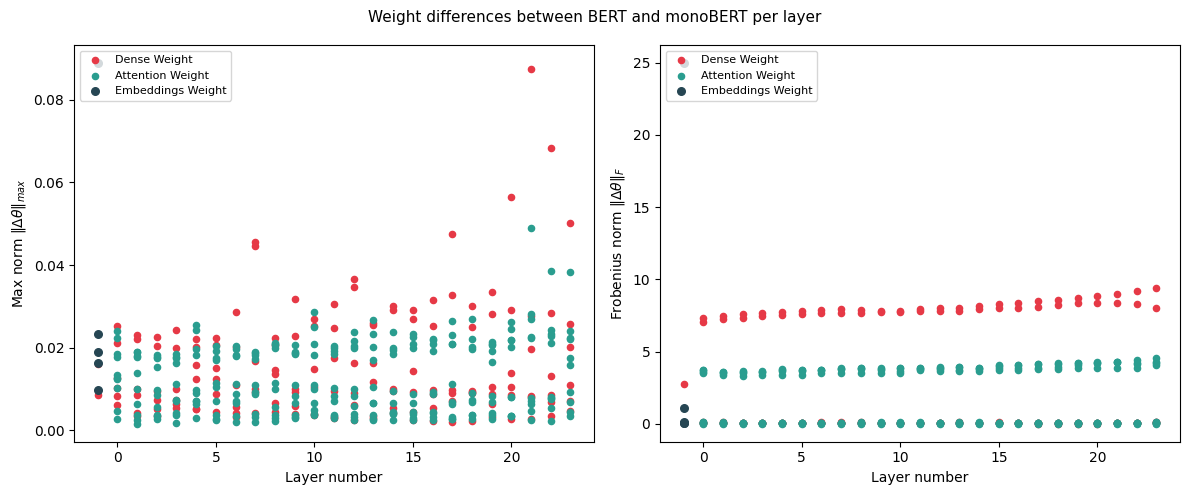
\includegraphics[width=0.92\textwidth]{figures/matrix_change_analysis.png}
    \caption{Matrix-level parameter differences between BERT and MonoBERT. Frobenius norm measures the overall magnitude of change, while max norm measures the largest individual weight difference. The observed changes motivate the selected attention-matrix adaptation experiments.}
    \label{fig:matrix_change_analysis}
\end{figure}

\FloatBarrier

Figure~\ref{fig:embedding_distance_analysis} reports embedding-level differences between BERT and MonoBERT using Euclidean distance and cosine similarity. The analysis was used to select the six embedding rows with the largest observed changes for the top-6 embedding experiment.

\begin{figure}[H]
    \centering
    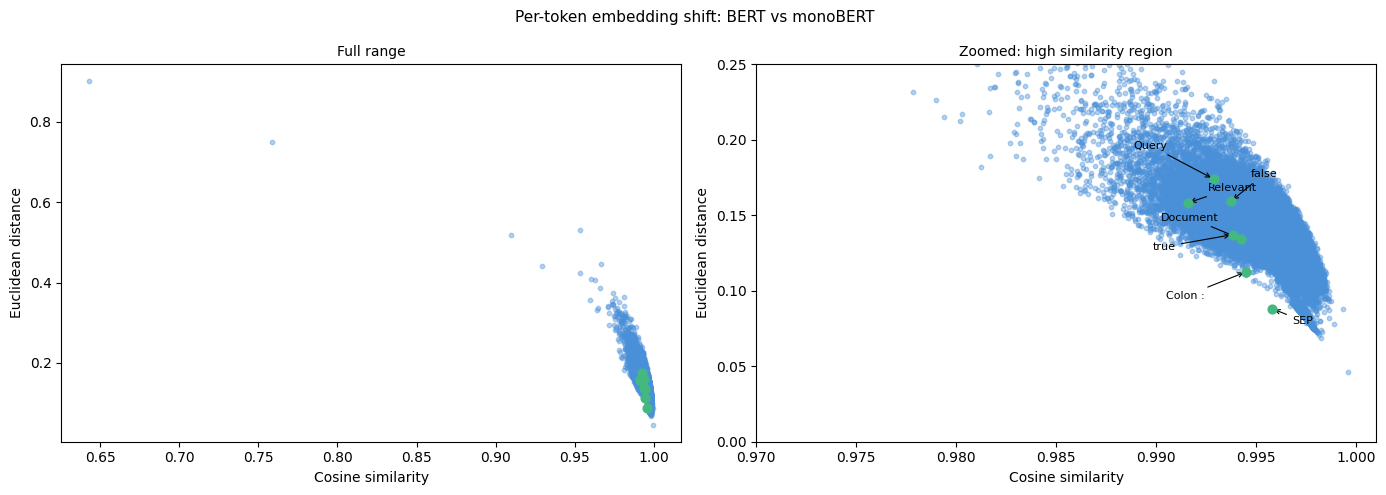
\includegraphics[width=0.92\textwidth]{figures/embedding_distance_analysis.png}
    \caption{Embedding-level differences between BERT and MonoBERT. Each point represents a vocabulary embedding vector. Euclidean distance measures magnitude of change, while cosine similarity measures directional change. The analysis motivates the selected embedding experiments.}
    \label{fig:embedding_distance_analysis}
\end{figure}

\FloatBarrier

\section{Overall Results}
\label{sec:results_overview}

The evaluation covers ten approaches across four datasets: TREC DL 2019, TREC DL 2020, MS MARCO dev small, and DL-Hard. The main metric discussed is nDCG@10 because it measures ranking quality at the top of the result list, which is the most important part of the ranking in a re-ranking setting. MRR@10, MAP@1000, and Recall@100 are also reported.

\begin{table}[ht]
\centering
\small
\begin{tabular}{lrcccc}
\hline
\textbf{Approach} & \textbf{Params} & \textbf{DL19} & \textbf{DL20} & \textbf{Dev Small} & \textbf{DL-Hard} \\
\hline
BM25 & 0 & 0.4138 & 0.4475 & 0.2302 & 0.2513 \\
CLS/SEP embeddings & 2,048 & 0.0449 & 0.0224 & 0.0093 & 0.0031 \\
Top-6 embeddings & 6,144 & 0.0197 & 0.0193 & 0.0054 & 0.0016 \\
LoRA top-3 attention & 49,152 & 0.5266 & 0.4825 & 0.2955 & 0.2873 \\
LoRA all attention & 1,572,864 & \textbf{0.6595} & 0.6762 & 0.4207 & \textbf{0.4006} \\
Top-3 attention matrices & 3,145,728 & 0.5627 & 0.5312 & 0.3348 & 0.3065 \\
All embeddings except CLS/SEP & 31,252,480 & 0.0274 & 0.0123 & 0.0066 & 0.0006 \\
All embeddings & 31,254,528 & 0.0510 & 0.0450 & 0.0173 & 0.0151 \\
Full MonoBERT & 335,143,938 & 0.6286 & 0.6426 & 0.4059 & 0.3977 \\
Public MonoBERT & --\textsuperscript{*} & 0.6540 & 0.6856 & 0.4297 & 0.3965 \\
\hline
\end{tabular}
\caption{nDCG@10 results across all evaluated approaches and datasets, ordered by number of trained parameters, from BM25 (no neural parameters) to full fine-tuning. The BM25 baseline is recomputed directly with PyTerrier over the MS MARCO passage index. \textsuperscript{*}Public MonoBERT is an externally released checkpoint and was not trained locally.}
\label{tab:results_nDCG}
\end{table}

\begin{table}[ht]
\centering
\small
\begin{tabular}{lrcccc}
\hline
\textbf{Approach} & \textbf{Params} & \textbf{DL19} & \textbf{DL20} & \textbf{Dev Small} & \textbf{DL-Hard} \\
\hline
BM25 & 0 & 0.4422 & 0.5056 & 0.6772 & 0.4007 \\
CLS/SEP embeddings & 2,048 & 0.1379 & 0.1202 & 0.1735 & 0.0475 \\
Top-6 embeddings & 6,144 & 0.0462 & 0.0306 & 0.0356 & 0.0112 \\
LoRA top-3 attention & 49,152 & 0.4669 & 0.5254 & 0.7433 & 0.4708 \\
LoRA all attention & 1,572,864 & \textbf{0.5229} & 0.5552 & 0.7890 & 0.5059 \\
Top-3 attention matrices & 3,145,728 & 0.4707 & 0.5331 & 0.7635 & 0.4741 \\
All embeddings except CLS/SEP & 31,252,480 & 0.1370 & 0.1655 & 0.2057 & 0.1244 \\
All embeddings & 31,254,528 & 0.3230 & 0.3291 & 0.5566 & 0.3321 \\
Full MonoBERT & 335,143,938 & 0.4706 & 0.5310 & 0.7809 & 0.4863 \\
Public MonoBERT & --\textsuperscript{*} & 0.5224 & \textbf{0.5680} & \textbf{0.7929} & \textbf{0.5217} \\
\hline
\end{tabular}
\caption{Recall@100 results across all evaluated approaches and datasets, ordered by number of trained parameters, from BM25 (no neural parameters) to full fine-tuning. \textsuperscript{*}Public MonoBERT is an externally released checkpoint and was not trained locally.}
\label{tab:results_recall}
\end{table}

\begin{table}[ht]
\centering
\small
\begin{tabular}{llcccc}
\hline
\textbf{Approach} & \textbf{Metric} & \textbf{DL19} & \textbf{DL20} & \textbf{Dev Small} & \textbf{DL-Hard} \\
\hline
Public MonoBERT & MRR@10 & \textbf{0.9814} & 0.9250 & \textbf{0.3706} & 0.6335 \\
LoRA all attention & MRR@10 & 0.9709 & \textbf{0.9414} & 0.3619 & 0.6712 \\
Full MonoBERT & MRR@10 & 0.9690 & 0.9290 & 0.3453 & \textbf{0.6815} \\
\hline
Public MonoBERT & MAP@1000 & \textbf{0.4722} & \textbf{0.4718} & \textbf{0.3730} & 0.2676 \\
LoRA all attention & MAP@1000 & 0.4697 & 0.4686 & 0.3651 & \textbf{0.2761} \\
Full MonoBERT & MAP@1000 & 0.4248 & 0.4285 & 0.3488 & 0.2585 \\
\hline
\end{tabular}
\caption{MRR@10 and MAP@1000 for the strongest neural re-rankers.}
\label{tab:results_mrr_map_best}
\end{table}

The results show a clear separation between embedding-only adaptation methods and methods that modify transformer attention or perform broader model adaptation. The strongest-performing approaches are Public MonoBERT, Full MonoBERT, and LoRA applied to all attention matrices. In contrast, all embedding-only methods perform substantially worse, even when the full embedding layer is trained.

\section{BM25 and MonoBERT Baselines}
\label{sec:results_baselines}

BM25 serves as the lexical baseline. Its performance is substantially lower than the neural re-ranking models across all datasets, achieving nDCG@10 scores of 0.4138 on TREC DL 2019, 0.4475 on TREC DL 2020, 0.2302 on MS MARCO dev small, and 0.2513 on DL-Hard. Although its absolute performance on DL-Hard remains modest, BM25 performs relatively better than several embedding-based approaches. This is likely because the DL-Hard candidate set was originally generated using BM25, making the evaluation pool inherently aligned with its retrieval strategy.

Public MonoBERT substantially outperforms BM25 on every dataset, which shows the effectiveness of neural cross-encoder re-ranking. The improvements are particularly pronounced on TREC DL 2019 and TREC DL 2020, where it achieves nDCG@10 scores of 0.6540 and 0.6856, respectively. These results highlight the advantage of full query-passage interaction within the BERT architecture.

Full MonoBERT is included to verify that the locally trained implementation produces results comparable to the publicly released model. Across all datasets, its performance closely matches that of Public MonoBERT, although the public model consistently achieves slightly higher scores. Full MonoBERT attains nDCG@10 values of 0.6286 on TREC DL 2019, 0.6426 on TREC DL 2020, 0.4059 on MS MARCO dev small, and 0.3977 on DL-Hard. The similarity between the two models indicates that the local training and evaluation pipeline is functioning as expected.

\section{Embedding-Level Adaptation}
\label{sec:results_embedding}

The main proposed approach trains only the embeddings of \texttt{[CLS]} and \texttt{[SEP]}. This updates only 2048 parameters, making it the smallest neural adaptation method in the thesis. However, the ranking performance is weak. It obtains nDCG@10 values of 0.0449 on TREC DL 2019, 0.0224 on TREC DL 2020, 0.0093 on MS MARCO dev small, and 0.0031 on DL-Hard.

These results show that the special-token embeddings alone are not sufficient to adapt BERT-large into an effective passage re-ranker. The result is important because it directly addresses the main transfer question from Light-MonoT5 to MonoBERT. Although \texttt{[CLS]} and \texttt{[SEP]} are structurally important in BERT, updating their embeddings does not provide enough control over the internal query-passage interaction behavior of the model.

The top-6 embedding experiment performs even weaker in most cases. This experiment was motivated by the embedding distance analysis between BERT and MonoBERT. However, during training, only four of the six selected embedding rows changed. The remaining selected tokens did not appear in the tokenized training inputs and therefore did not receive gradient updates. This reveals a practical limitation of selected embedding tuning: selecting an embedding row is not sufficient if the corresponding token is rare or absent during training.

The all-embedding experiment provides a more informative comparison. It trains the entire embedding matrix while freezing the rest of the model. This approach improves Recall@100 substantially in some cases, especially on MS MARCO dev small where it reaches 0.5566. However, its nDCG@10 remains low. This suggests that embedding adaptation can move some relevant passages higher in the ranking, but it does not learn the fine-grained ordering needed for strong top-10 performance.

The all-embeddings-except-\texttt{[CLS]}/\texttt{[SEP]} experiment also performs poorly. This indicates that ordinary vocabulary embeddings alone are not sufficient to adapt the frozen model. It also provides an indirect contrast with the \texttt{[CLS]}/\texttt{[SEP]} experiment: the structural tokens appear to contribute more than ordinary vocabulary embeddings, but neither structural-token tuning nor non-structural embedding tuning is sufficient on its own.

Overall, the embedding-level experiments show that embeddings are too limited as the sole adaptation mechanism for MonoBERT-style re-ranking. They influence the initial token representations, but they do not directly modify the internal transformer computations responsible for modeling query-passage interactions.

\section{Attention-Based Adaptation}
\label{sec:results_attention}

The attention-based methods perform substantially better than the embedding-only methods. The top-3 attention matrix experiment trains the three matrices that changed most in the BERT-to-MonoBERT analysis. It achieves nDCG@10 values of 0.5627 on TREC DL 2019 and 0.5312 on TREC DL 2020, while also performing strongly on MS MARCO dev small and DL-Hard.

This result provides evidence that the parameter-change analysis successfully identified attention matrices that are important for retrieval adaptation. The selected matrices were not chosen randomly; rather, they were selected because they exhibited the largest changes between BERT and MonoBERT. Their strong performance supports the hypothesis that the analysis identified parts of the model that play an important role in IR adaptation.

The results also support a broader interpretation that passage re-ranking relies heavily on attention-level interactions. Since cross-encoders allow query and passage tokens to interact through self-attention, modifying attention matrices directly affects one of the primary mechanisms responsible for relevance matching. This likely explains why attention-matrix tuning performs substantially better than embedding-only tuning.

An interesting comparison is between direct tuning of the selected attention matrices and applying LoRA to the same matrices. Direct optimization consistently achieves higher effectiveness than LoRA top-3 attention, reaching nDCG@10 scores of 0.5627 versus 0.5266 on TREC DL 2019 and 0.5312 versus 0.4825 on TREC DL 2020. This suggests that, for a very small subset of attention modules, directly updating the original parameters is more effective than constraining the updates to low-rank adapters, although LoRA remains considerably more parameter-efficient.

\section{LoRA Results}
\label{sec:results_lora}

LoRA applied to all attention matrices is the strongest parameter-efficient method evaluated in this thesis. It performs comparably to both Public MonoBERT and Full MonoBERT across all datasets. On TREC DL 2019, it achieves an nDCG@10 of 0.6595, slightly exceeding both Public MonoBERT (0.6540) and Full MonoBERT (0.6286). On TREC DL 2020, it reaches 0.6762, remaining close to Public MonoBERT's 0.6856.

These results show that LoRA is a strong PEFT baseline for passage re-ranking. By adapting the attention computations without updating the full set of model parameters, it preserves most of the effectiveness of full fine-tuning while requiring substantially fewer trainable parameters.

LoRA top-3 attention performs worse than LoRA all attention, but remains competitive relative to its parameter count. It achieves nDCG@10 scores of 0.5266 on TREC DL 2019 and 0.4825 on TREC DL 2020, while also maintaining strong Recall@100 values across the evaluated datasets. This indicates that applying LoRA only to the most important attention matrices can retain a substantial portion of the performance achieved by broader LoRA adaptation.

The comparison between LoRA all attention and LoRA top-3 attention is particularly relevant to the thesis. It suggests that parameter-change analysis can guide not only direct parameter tuning, but also the placement of parameter-efficient adaptation modules. Rather than applying LoRA uniformly across all attention layers, the results indicate that concentrating adaptation on a small number of carefully selected modules remains an effective strategy.

\section{Efficiency and Parameter Trade-offs}
\label{sec:results_efficiency}

The experiments show that the number of trainable parameters alone does not determine ranking performance. The \texttt{[CLS]}/\texttt{[SEP]} experiment is extremely parameter-efficient, yet its ranking effectiveness is poor. Conversely, the all-embedding experiment trains substantially more parameters than the \texttt{[CLS]}/\texttt{[SEP]} approach but still performs considerably worse than the attention-based methods.

These results suggest that the location of adaptation is more important than the number of trainable parameters alone. Parameters within the attention layers have a much greater influence on ranking effectiveness because they largely determine how query and passage tokens interact throughout the transformer. In contrast, embedding parameters affect only the initial token representations before they are processed by the frozen transformer layers.

The top-3 attention and LoRA top-3 attention experiments provide a useful compromise between parameter efficiency and ranking effectiveness. Although they update only a small fraction of the model compared with full fine-tuning or LoRA all attention, they substantially outperform all embedding-only approaches. This indicates that carefully selected attention modules constitute effective adaptation targets for BERT-based passage re-ranking.

\begin{table}[ht]
\centering
\small
\resizebox{\textwidth}{!}{%
\begin{tabular}{l r p{6.5cm}}
\hline
\textbf{Approach} & \textbf{Updated Parameters} & \textbf{Main Updated Component} \\
\hline
BM25 & 0 & No neural parameters \\
Public MonoBERT & -- & Public fully fine-tuned model \\
CLS/SEP embeddings & 2,048 & Two special-token embeddings \\
Top-6 embeddings & 6,144 & Six selected embedding rows \\
Top-3 attention matrices & 3,145,728 & Three full attention matrices \\
All embeddings & 31,254,528 & Full word embedding matrix \\
All embeddings except CLS/SEP & 31,252,480 & Word embeddings except token IDs 101 and 102 \\
LoRA all attention & 1,572,864 & Low-rank adapters in all attention matrices \\
LoRA top-3 attention & 49,152 & Low-rank adapters in selected attention matrices \\
Full MonoBERT & 335,143,938 & All model parameters \\
\hline
\end{tabular}%
}
\caption{Number of updated parameters for each approach. The table highlights the efficiency-effectiveness trade-off between highly restricted embedding-level methods, attention-level methods, LoRA variants, and full fine-tuning.}
\label{tab:updated_parameters}
\end{table}

\section{Discussion}
\label{sec:results_interpretation}

The results clarify the relationship between Light-MonoT5 and MonoBERT. The Light-MonoT5 idea motivates the hypothesis that selected embeddings may control task-specific behavior. In the BERT setting, this hypothesis is only partially supported. Special-token embeddings can be trained successfully, and the gradient masking works as intended, but the resulting ranking model is not competitive with attention-based adaptation methods.

One possible explanation is the architectural difference between MonoT5 and MonoBERT. MonoT5 and MonoBERT use different mechanisms for relevance prediction. MonoT5 is a sequence-to-sequence model where prompt tokens can directly influence the generated output. In contrast, MonoBERT predicts relevance from the final \texttt{[CLS]} representation after multiple layers of self-attention. Therefore, changing only the initial \texttt{[CLS]} and \texttt{[SEP]} embeddings may not provide sufficient control over the final relevance prediction process.

The strongest evidence from the experiments is that attention-layer adaptation is substantially more effective than embedding-layer adaptation for BERT-based passage re-ranking. Attention matrices influence how query and passage tokens interact throughout the transformer layers. Since relevance depends on modelling relationships between the query and passage, modifying attention components appears to provide a more effective adaptation mechanism than modifying only the input embeddings.

\section{Answers to Research Questions}
\label{sec:results_rq}

\justifying

\begin{description}

\item[\textbf{RQ1}] \textbf{Can a BERT cross-encoder be adapted by training only selected embeddings?}

\vspace{-0.4\baselineskip}

Selected embeddings can be trained successfully, but the resulting ranking performance is weak. Therefore, embedding-only tuning is possible, but it is not competitive with attention-based adaptation methods.

\vspace{0.6\baselineskip}

\item[\textbf{RQ2}] \textbf{How does CLS/SEP tuning compare with top-changed embedding tuning?}

\vspace{-0.4\baselineskip}

The \texttt{[CLS]}/\texttt{[SEP]} method generally performs better than the top-6 embedding method, although both approaches remain substantially weaker than attention-based methods. The top-6 method is additionally limited by the fact that some selected embedding rows did not appear during training and therefore did not receive updates.

\vspace{0.6\baselineskip}

\item[\textbf{RQ3}] \textbf{Are useful changes concentrated more in embeddings or attention matrices?}

\vspace{-0.4\baselineskip}

The results indicate that attention matrices are substantially more effective adaptation targets than embeddings for BERT-based passage re-ranking.

\vspace{0.6\baselineskip}

\item[\textbf{RQ4}] \textbf{How does embedding-level tuning compare with LoRA?}

\vspace{-0.4\baselineskip}

LoRA is substantially stronger than embedding-level tuning. LoRA applied to all attention matrices performs close to MonoBERT, while embedding-only methods remain far below this level of effectiveness.

\vspace{0.6\baselineskip}

\item[\textbf{RQ5}] \textbf{Can LoRA on the top-3 changed matrices retain much of LoRA all attention performance?}

\vspace{-0.4\baselineskip}

Yes. LoRA top-3 attention performs worse than LoRA all attention, but it retains a substantial portion of the ranking effectiveness while requiring significantly fewer trainable parameters.

\vspace{0.6\baselineskip}

\item[\textbf{RQ6}] \textbf{Does Full MonoBERT validate the setup?}

\vspace{-0.4\baselineskip}

Yes. Full MonoBERT performs close to Public MonoBERT, indicating that the local training and evaluation pipeline is broadly aligned with MonoBERT-style passage re-ranking.

\end{description}


\section{Summary}
\label{sec:results_summary}

The main conclusion from the results is that embedding-level tuning is informative but not sufficient for strong BERT-based passage re-ranking. The most effective adaptation mechanisms evaluated in this thesis are attention-based. LoRA applied to all attention matrices performs close to MonoBERT, while LoRA top-3 attention and direct top-3 attention matrix tuning provide effective restricted alternatives with fewer trainable parameters.

Overall, the experiments suggest that adaptation location is more important than parameter count alone. Although embedding-level methods modify the input representation space, attention-level methods provide a more direct mechanism for modifying query-passage interaction behaviour, which is central to cross-encoder passage re-ranking.